\documentclass[12pt]{TDP005mall}
\usepackage{graphicx}


\newcommand{\version}{Version 1.0}
\author{Elliot Johansson, \url{elljo130@student.liu.se}\\
  Lukas Freyland, \url{lukfr510@student.liu.se}\\
  Nadim Lakrouz, \url{nadla777@student.liu.se}}
\title{Kravspecifikation}
\date{2022-11-10}
\rhead{Elliot Johansson\\
Lukas Freyland\\
Nadim Lakrouz}



\begin{document}
\projectpage
\section{Revisionshistorik}
\begin{table}[!h]
\begin{tabularx}{\linewidth}{|l|X|l|}
\hline
Ver. & Revisionsbeskrivning & Datum \\\hline
1.0 & första utkast & 2022-11-10 \\\hline
\end{tabularx}
\end{table}


\section{Spelide}

Spelet utspelas i en 2D-värld där kameraperspektivet är uppifrån. Spelarens mål är att bekämpa flera vågor av attackerande fiender genom att använda kombinationer av magiska formler. Formlerna grundas i fyra element som sedan kombineras för att skapa olika typer av attacker. Fiender kommer röra sig emot spelaren och när de är tillräckligt nära kommer de explodera. Vid explosionen tar spelaren skada och fienden dör. Bland fienderna finns det olika typer av fiender och beroende på vilken typ tar den fienden mer skada av ett element än vad de andra fienderna skulle göra.\\
De magiska formlerna kommer spelaren kunna göra genom olika inmatningar. Spelaren kommer använda en eller två element för varje formel. Varje formel kostar ''Mana'' vilket begränsar vilka formler som spelaren kan använda beroende på hur mycket mana spelaren har. Spelaren får tillbaka ''Mana'' då ''Man'' regenereras över tid. Det finns också en begränsning för att spelaren inte ska överanvända formler på en gång.
Spelaren kommer ha tillgång till att skapa olika magiska formler från början men kommer inte veta de olika kombinationerna för formeln och vad den gör. Så spelaren får testa sig fram och upptäcka alla formler själv. 


\subsection{Målgrupp}
Spelet är tänkt för unga personer som gillar action, strategi och att upptäcka nya saker.

\section{Spelupplevelse}
Spelaren får chansen att upptäcka själv vad hen kan göra för att bli bättre och klara sig längre. T.ex. då spelaren kommer lära sig flera nya magiska formler under varje spelomgång. 

\subsection{Spelmekanik}
Spelaren kommer inte kunna flytta runt men kommer kunna använda sig av de olika grundformlerna för att attackera, läka och skydda sig mot fiender.

\subsubsection{Knappar}
\begin{itemize}
\item Q - Vatten formel
\item W - Jord formel
\item E - Eld formel
\item R - Vind formel
\end{itemize}

\subsubsection{Grundläggande kombinationer}
\begin{itemize}
\item QQ - Vatten läknings formel
\item WW - Jord skölds formel
\item EE - Eld bolls formel
\item RR - Virvelvinds formel
\end{itemize}


\section{Regler}
\subsection{Spelplan}
En vertikal rektangel med fixerad storlek
\subsection{Spelare}
\begin{itemize}
\item Spelaren ser hela spelplanen
\item Spelaren står still
\item Spelaren kan kasta formler för att skada fiender och skydda sig själv.
\item Spelaren har ett visst antal liv
\item Spelaren har en viss mängd mana
\item När spelaren förlorat alla liv är spelet över
\end{itemize}
\subsection{poäng}
När spelaren dödar fiender får hen poäng.
\subsection{fiender}
Fienderna rör sig alltid mot spelaren och när den är inom räckhåll exploderar den och skadar spelaren med x antal damage. Fienderna har varierande livs poäng, hastighet och resistens mot element.
\section{visualisering}
\begin{center}
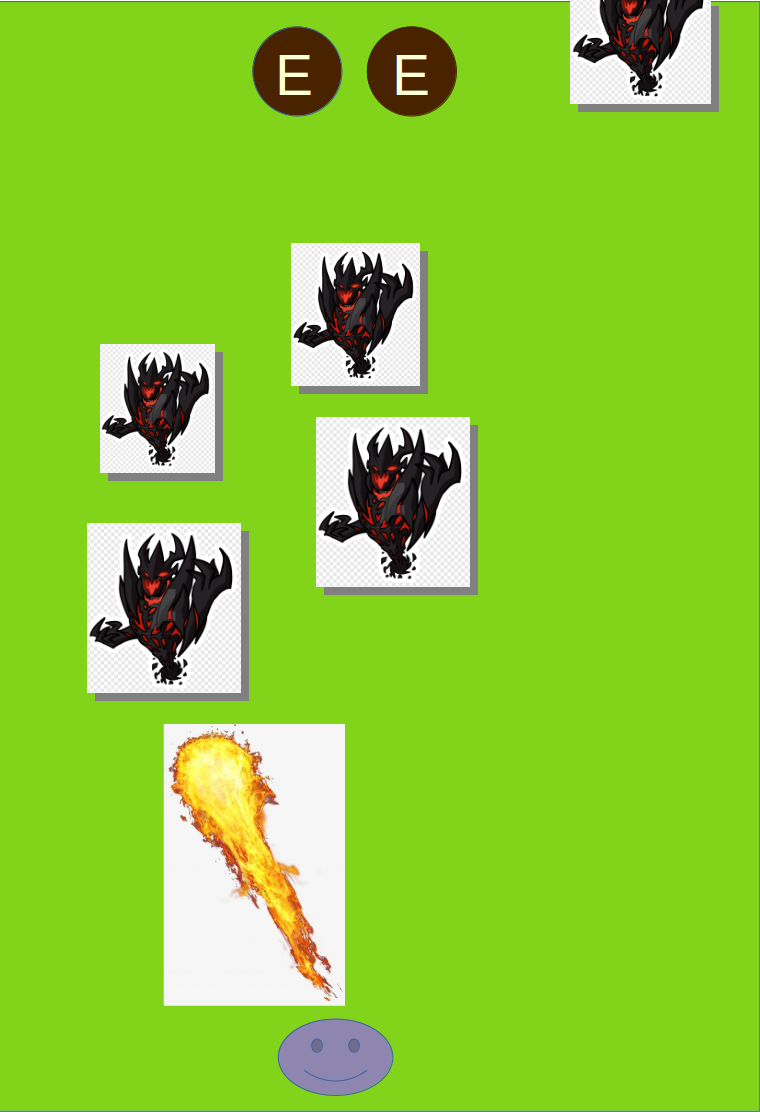
\includegraphics[scale=0.5]{spel.png}
\end{center}
\newpage

\section{Kravformulering}

\subsection{Ska-krav}
\begin{itemize}
\item Det ska finnas ett spelarobjekt
\item Det ska finnas ett fiendeobjekt
\item Det ska gå att göra formler
\item Grundformler ska finnas
\item Spelaren ska kunna ta skada
\item Spelaren ska kunna göra skada till fiender
\item Fiender ska kunna ta skada
\item Fiender ska kunna göra skada
\item Fiender ska alltid röra sig mot fienden
\item Det ska finnas en startmeny
\item Spelet ska vara över när spelaren har slut på liv
\item Det ska finnas en mana mätare töms vid användning av formler
\item Mana ska regenerera över tid
\item poäng räknare
\end{itemize}

\subsection{Bör-krav}
\begin{itemize}
\item Flera kombinationer av formler och flera element.
\item Spara poäng
\end{itemize}

\end{document}
